\documentclass[12pt,a4paper]{article}

\usepackage[utf8]{inputenc}
\usepackage[T1]{fontenc}
\usepackage[brazil]{babel}
\usepackage{graphicx}
\usepackage{geometry}
\usepackage{amsmath}
\usepackage{amssymb}
\usepackage{indentfirst}
\usepackage{hyperref}
\usepackage{listings}
\usepackage{float}
\usepackage{caption}


\geometry{
  left=3cm,
  right=3cm,
  top=3cm,
  bottom=2cm
}

\begin{document}
\begin{titlepage}
\begin{center}


\includegraphics[width=2.5cm]{logo ufal.png}\\[0.5cm]

\textbf{UNIVERSIDADE FEDERAL DE ALAGOAS}\\[0.2cm]
SISTEMAS DE CONTROLE INTELIGENTE\\[0.2cm]
ENGENHARIA DE COMPUTAÇÃO

\vfill

{\Large \textbf{Ajuste Automático de Controladores PID Usando Métodos de Otimização Inteligente}}


\vfill

Jose Anderson Da Silva\\
Thiago Fellype Marques\\
Pedro Henrique Vieira Gilo\\
Caio Oliveira Franca Dos Anjos\\
Alasson De Araujo Alves

\vfill

MACEIÓ -- AGOSTO, 2025

\end{center}
\end{titlepage}

\tableofcontents
\newpage

\section{Índice de Desempenho Goodhart}

Os algoritmos de sintonia inteligente utilizados neste trabalho (Nelder--Mead, Algoritmo Genético e PSO) não atuam diretamente sobre indicadores simples, como o erro absoluto ou o MSE. Em vez disso, todos otimizam um único índice de desempenho, denominado \emph{Índice de Goodhart}, que agrega em uma forma escalar diferentes aspectos desejáveis do comportamento do controlador PID.

\subsection{Visão Geral}

A ideia central do índice de Goodhart é avaliar simultaneamente:
\begin{itemize}
    \item o esforço médio aplicado pelo controlador sobre o atuador;
    \item o quão suave (ou oscilatória) é a ação de controle ao longo do tempo;
    \item o erro entre o setpoint e a variável de processo.
\end{itemize}

Dessa forma, evita-se que o algoritmo de otimização busque apenas reduzir o erro a qualquer custo, o que poderia resultar em comandos muito agressivos, saturações frequentes ou desgaste prematuro do atuador.

\subsection{Formulação Matemática}

O índice é escrito como uma combinação linear ponderada:
\begin{equation}
    G = c_1 \epsilon_1 + c_2 \epsilon_2 + c_3 \epsilon_3,
\end{equation}
em que $c_1$, $c_2$ e $c_3$ são pesos ajustáveis e os termos $\epsilon_i$ são definidos a seguir.

\subsubsection*{1. Esforço Médio da Ação de Controle}

\begin{equation}
    \epsilon_1 = \frac{1}{N}\sum_{k=1}^{N} SC_k,
\end{equation}
onde $SC_k$ representa o valor da ação de controle no instante discreto $k$. Este termo mede o \emph{nível médio} do sinal de controle, associado ao consumo de energia ou ao esforço constante sobre o atuador.

\subsubsection*{2. Variabilidade da Ação de Controle}

\begin{equation}
    \epsilon_2 = \frac{1}{N}\sum_{k=1}^{N} (SC_k - \epsilon_1)^2,
\end{equation}
que corresponde à variância do sinal de controle. Valores elevados de $\epsilon_2$ indicam comandos muito oscilatórios ou com \emph{jitter}, o que pode causar desgaste mecânico e ruído.

\subsubsection*{3. Erro Quadrático Médio}

\begin{equation}.
    \epsilon_3 = \frac{1}{N}\sum_{k=1}^{N} e_k^2,
\end{equation}
onde $e_k$ é o erro entre o setpoint e a variável de processo. Este termo é o erro quadrático médio clássico, garantindo que o desempenho em rastreamento continue sendo levado em consideração.

\subsection{Significado dos Pesos}

Os pesos $c_1$, $c_2$ e $c_3$ definem a ``personalidade'' do controlador resultante, permitindo privilegiar economia, suavidade ou precisão, conforme resumido na Tabela~\ref{tab:pesos}.

\begin{center}
\begin{tabular}{|c|c|c|}
\hline
\textbf{Peso} & \textbf{Influência} & \textbf{Aplicação típica} \\
\hline
$c_1$ & Esforço médio & Economia de energia, limitação de atuador \\
$c_2$ & Suavidade     & Redução de jitter, desgaste mecânico e ruído \\
$c_3$ & Precisão      & Rastreamento rigoroso do setpoint \\
\hline
\end{tabular}
\captionof{table}{Interpretação dos pesos do índice de Goodhart.}
\label{tab:pesos}
\end{center}

Neste relatório foram analisadas, principalmente, duas configurações:
\begin{itemize}
    \item $(c_1, c_2, c_3) = (0{,}33,\;0{,}33,\;0{,}34)$: pesos aproximadamente equilibrados, com prioridade ligeiramente maior à precisão;
    \item $(c_1, c_2, c_3) = (0{,}01,\;0{,}01,\;0{,}98)$: quase todo o peso concentrado no erro, privilegiando o rastreamento mesmo ao custo de maior esforço de controle.
\end{itemize}

\subsection{Definição no Código}

A parametrização dos pesos no código é realizada na criação do objeto \texttt{PIDAutoTunning}, por exemplo:
\begin{verbatim}
auto_tunning = PIDAutoTunning(dc_motor_model,
                              goodhart_gains=[0.33, 0.33, 0.34])
parcial_result = auto_tunning.tunning(initial_set, False)
parcial_result = sorted(parcial_result, key=lambda x: x[1])
\end{verbatim}

\newpage

\section{Sintonia via Método de Nelder--Mead}

O método de Nelder--Mead é um algoritmo de otimização numérica \emph{derivative-free}, ou seja, não necessita do cálculo explícito de gradientes. Ele trabalha com um \emph{simplex} no espaço de parâmetros, avaliando sucessivas combinações de ganhos $(K_p, K_i, K_d)$ até aproximar um mínimo local do índice de Goodhart.

\subsection{Configuração com Pesos Balanceados \\ $(c_1,c_2,c_3) = (0{,}33,0{,}33,0{,}34)$}

\subsubsection{Setpoint Degrau}

Neste caso, foi utilizado um setpoint em degrau e saturação do controlador em $[-255,\,255]$.
O tempo total da simulação para a otimização foi de aproximadamente $905{,}12$ segundos.

\begin{figure}[ht]
    \centering
    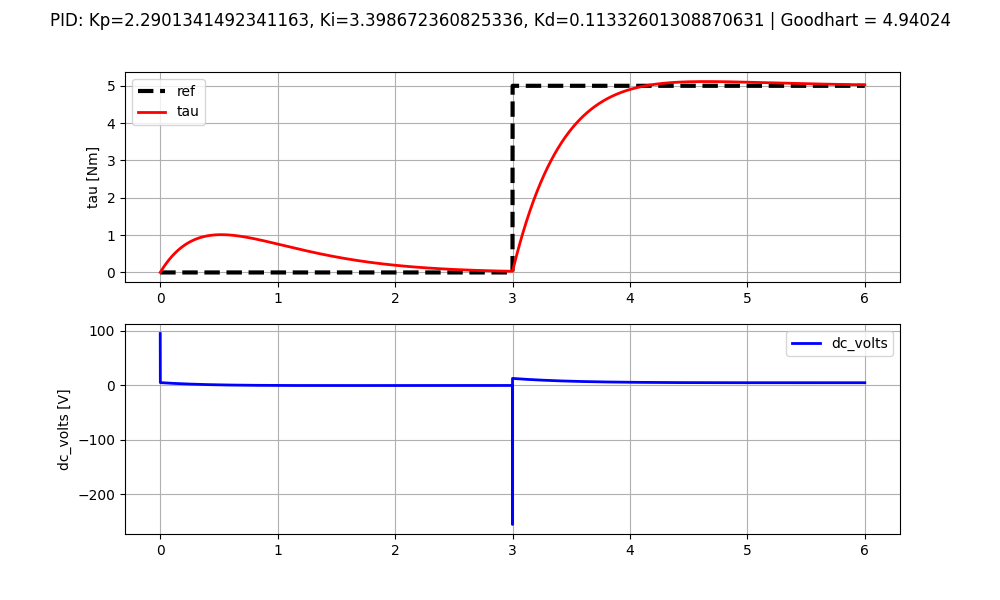
\includegraphics[width=0.8\linewidth]{Nelder Mead degrau.png}
    \caption{Resposta do sistema para o método de Nelder--Mead com setpoint degrau.}
    \label{fig:nelder-step}
\end{figure}


\begin{verbatim}
Tempo total de execução: 905.119 segundos
Optimization successful: False
Message: Maximum number of function evaluations has been exceeded.
Optimal parameters (x): [2.29013415 3.39867236 0.11332601]
Minimum function value (fun): 4.940238
Number of function evaluations (nfev): 120
\end{verbatim}

Observa-se que o método atingiu uma região de custo relativamente baixo (Goodhart $\approx$ 4.94, porém o critério interno de parada relacionado ao número máximo de avaliações foi excedido antes de declarar convergência formal. Ainda assim, os ganhos encontrados resultam em uma ação de controle moderada e um compromisso razoável entre erro, esforço e suavidade.

\subsubsection{Setpoint Cosseno}

Foi também avaliado um setpoint variante no tempo em forma de cosseno. O tempo de simulação foi de $928{,}32$ segundos.

\begin{center}
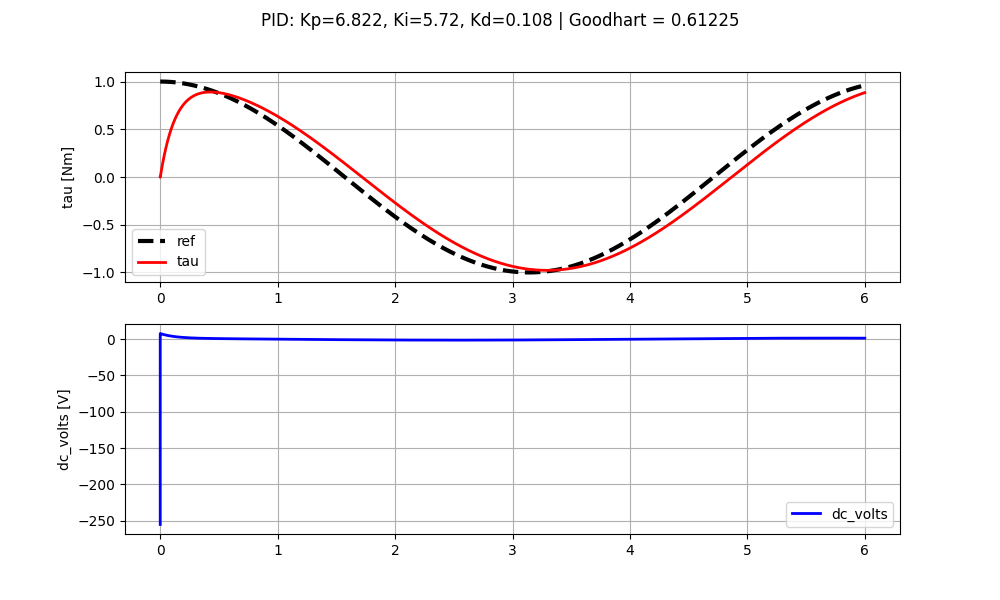
\includegraphics[width=11cm]
{Nelder Mead coseno.png}
\end{center}

\begin{verbatim}
Tempo total de execução: 928.324 segundos
Optimization successful: False
Message: Maximum number of function evaluations has been exceeded.
Optimal parameters (x): [6.822 5.72  0.108]
Minimum function value (fun): 0.612252
Number of function evaluations (nfev): 120
\end{verbatim}

O valor de Goodhart diminui para cerca de $0{,}61$, indicando melhora significativa em relação ao caso com degrau. Neste cenário, a dinâmica do setpoint exige um controlador mais responsivo, o que se reflete em ganhos proporcionais e integrais maiores.

\subsection{Configuração com Ênfase no Erro \\ $(c_1,c_2,c_3) = (0{,}01,0{,}01,0{,}98)$}

\subsubsection{Setpoint Degrau}

Ao concentrar quase todo o peso em $c_3$, o algoritmo passa a privilegiar fortemente o erro quadrático médio, mesmo que isso aumente o esforço de controle.

\begin{center}
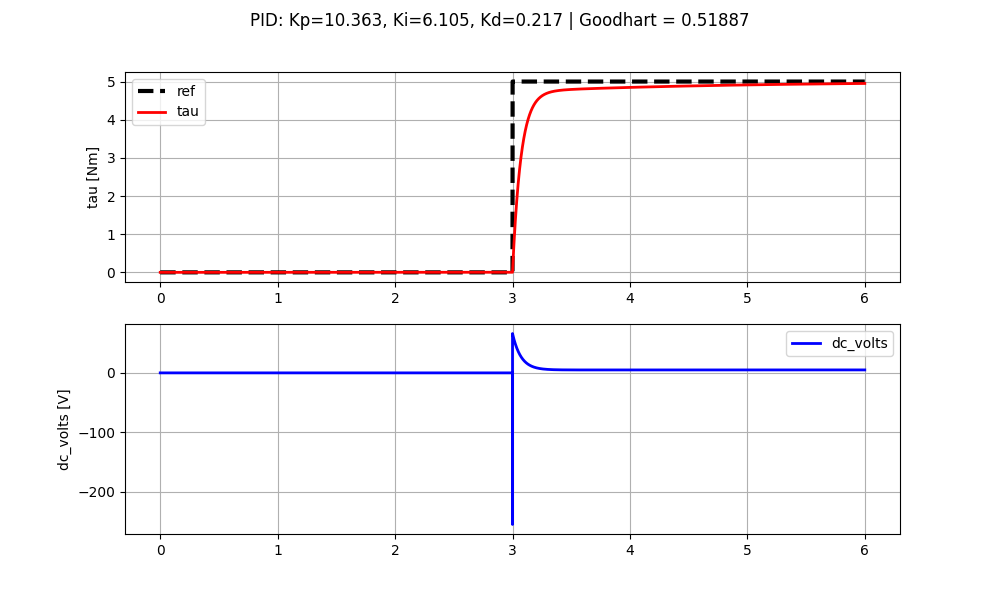
\includegraphics[width=11cm]{Nelder_Mead_gains_degrau.png}
\end{center}

\begin{verbatim}
Tempo total de execução: 342.475 segundos
Optimization successful: True
Message: Optimization terminated successfully.
Optimal parameters (x): [10.363  6.105  0.217]
Minimum function value (fun): 0.518869
Number of function evaluations (nfev): 46
\end{verbatim}

Neste caso, a convergência foi declarada com sucesso em um número reduzido de avaliações. Os ganhos $K_p$ e $K_i$ aumentam consideravelmente, o que leva a uma resposta mais agressiva e menor erro estacionário, coerente com a ponderação escolhida.

\subsubsection{Setpoint Cosseno}

\begin{center}
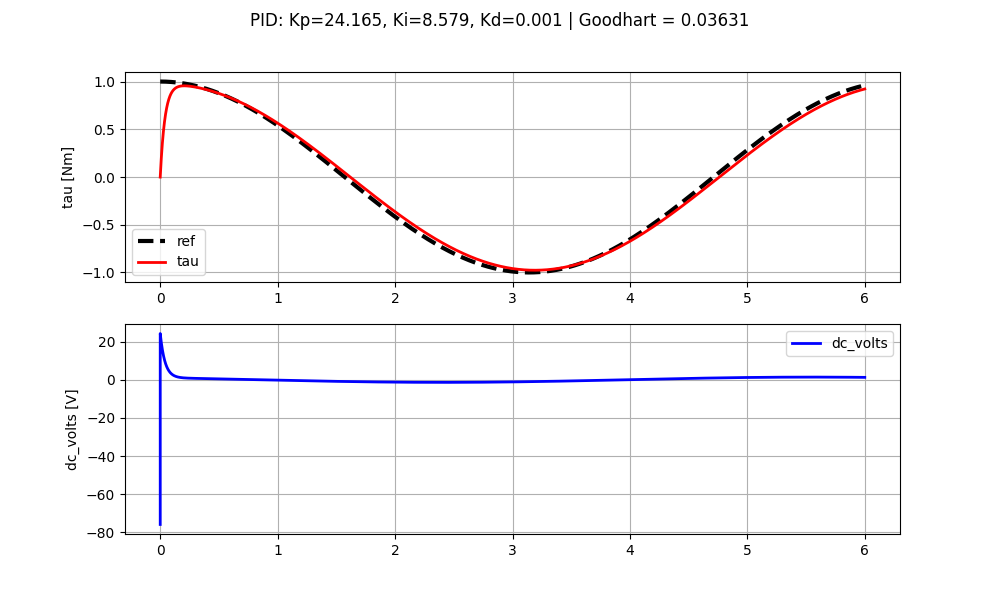
\includegraphics[width=11cm]{Nelder_Mead_gains_cosseno.png}
\end{center}

\begin{verbatim}
Tempo total de execução: 343.944 segundos
Optimization successful: True
Message: Optimization terminated successfully.
Optimal parameters (x): [2.4165e+01 8.5790e+00 1.0000e-03]
Minimum function value (fun): 0.036308
Number of function evaluations (nfev): 47
\end{verbatim}

O índice de Goodhart atinge valores da ordem de $10^{-2}$, indicando excelente rastreamento mesmo para setpoint oscilatório. O ganho proporcional se torna elevado ($K_p \approx 24$), acompanhado de um termo integral dominante, enquanto o ganho derivativo tende praticamente a zero.

\newpage
\section{Sintonia via  Genético}

O Algoritmo Genético (GA) busca a solução ótima por meio de operadores inspirados em evolução biológica, como seleção, cruzamento e mutação. Cada indivíduo da população representa um vetor de ganhos $(K_p,K_i,K_d)$, avaliado pelo índice de Goodhart.

\subsection{Pesos Balanceados $(0{,}33,0{,}33,0{,}34)$}

\subsubsection*{Setpoint Degrau}

\begin{figure}[H]
    \centering
    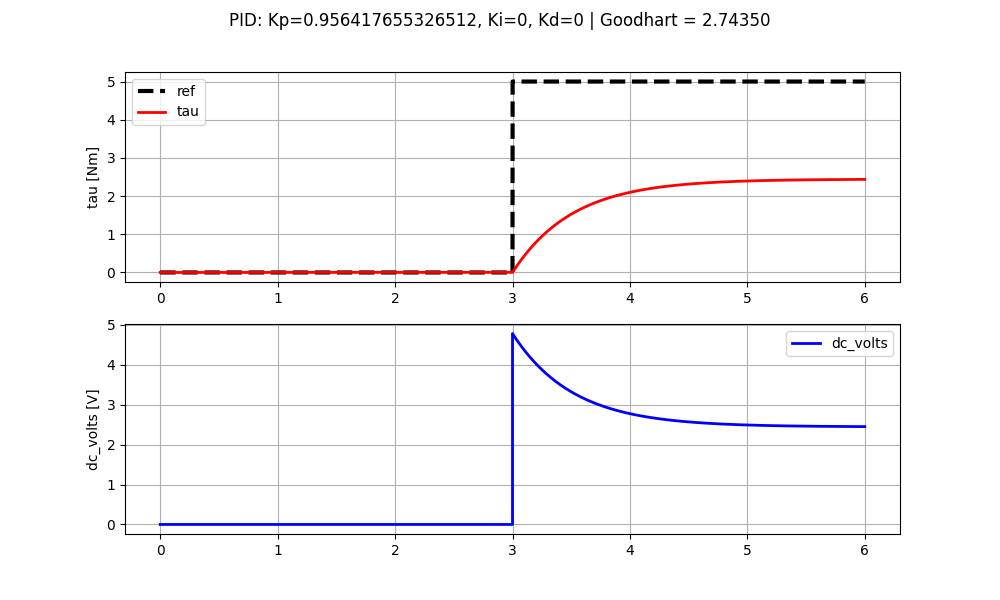
\includegraphics[width=0.8\linewidth]{genetico_degrau.png}
    \caption{Resposta para o método Genético com setpoint degrau.}
    \label{fig:ga-degrau}
\end{figure}


\begin{verbatim}
Tempo total de execução: 392.336 segundos
Melhor solução encontrada:
Kp = 0.956417655326512
Ki = 0
Kd = 0
Custo = 2.743498
\end{verbatim}

O GA encontrou como melhor solução um controlador puramente proporcional, com $K_i = K_d = 0$. 
O custo ainda é relativamente alto (Goodhart $\approx$ 2.74), indicando que, sob esses pesos, 
o espaço de busca poderia ser explorado por mais gerações ou com parametrizações diferentes 
para melhorar o compromisso entre erro e suavidade.


\subsection{Ênfase no Erro $(0{,}01,0{,}01,0{,}98)$}

\subsubsection*{Setpoint Degrau}

\begin{center}
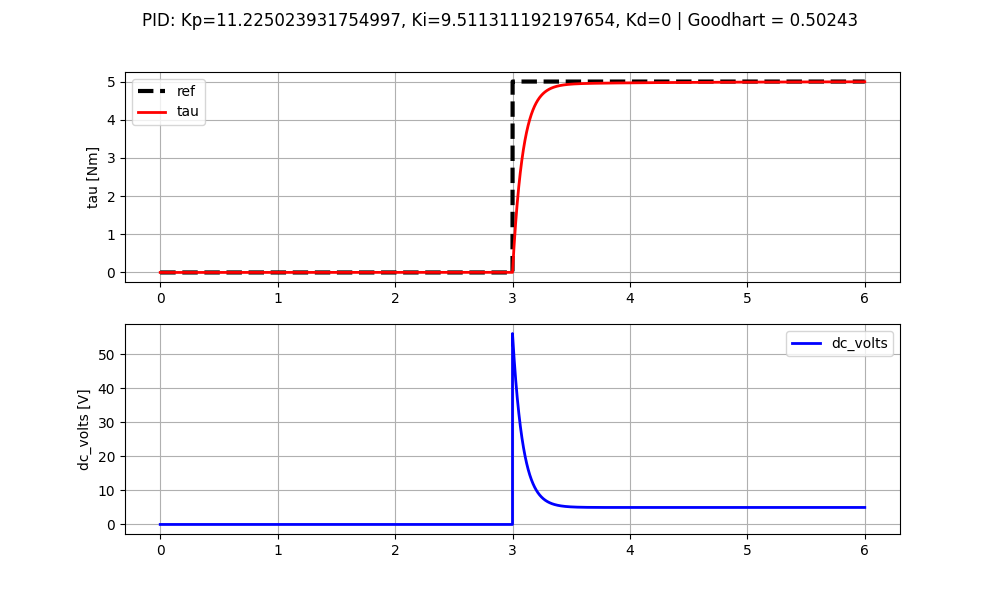
\includegraphics[width=11cm]{genetico_cosseno.png}
\end{center}

\begin{verbatim}
Tempo total de execução: 168.229 segundos
Melhor solução encontrada:
Kp = 11.225023931754997
Ki = 9.511311192197654
Kd = 0
Custo = 0.502428
\end{verbatim}

Com maior peso em $c_3$, o GA passa a privilegiar diretamente a redução do erro, o que leva a um controlador com ganhos proporcional e integral elevados, ainda sem componente derivativa. O custo final é compatível com o obtido por Nelder--Mead na mesma configuração de pesos, reforçando a validade do índice adotado.

\newpage

\section{Sintonia via PSO (Particle Swarm Optimization)}

O método PSO modela um enxame de partículas que navegam pelo espaço de parâmetros, atualizando suas posições de acordo com a melhor experiência individual e coletiva. Cada partícula representa um conjunto de ganhos $(K_p,K_i,K_d)$ avaliado pela mesma função de custo.

\subsection{Pesos Balanceados $(0{,}33,0{,}33,0{,}34)$}

\subsubsection*{Setpoint Degrau}

\begin{center}
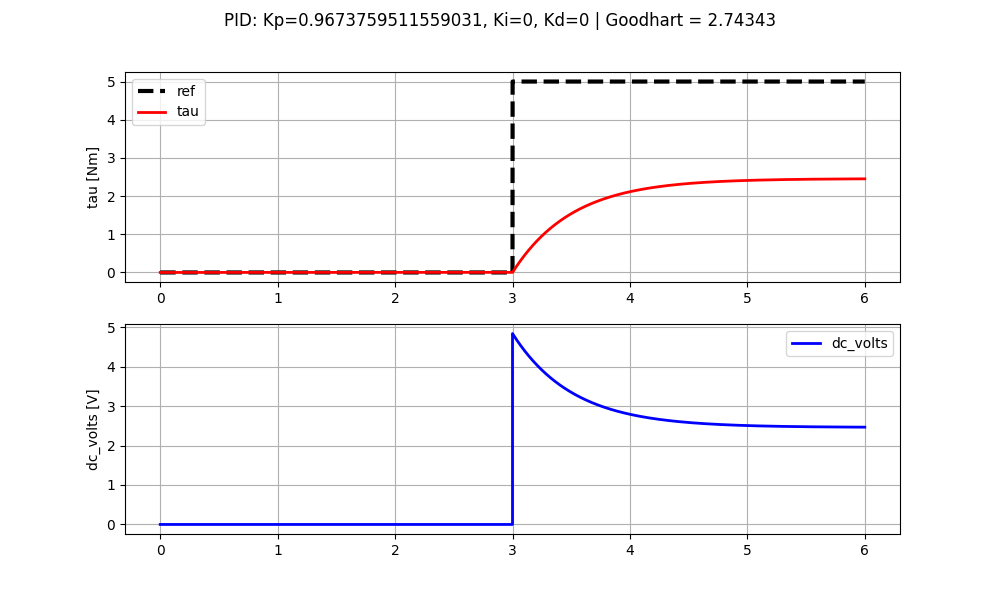
\includegraphics[width=11cm]{pso_degrau.png}
\end{center}

\begin{verbatim}
Tempo total de execução: 765.576 segundos
Melhor solução encontrada:
Kp = 0.9674
Ki = 0.0000
Kd = 0.0000
Custo = 2.743434
\end{verbatim}

O PSO converge para uma solução muito semelhante à obtida pelo Algoritmo Genético nesta configuração de pesos, também com controlador proporcional puro. O custo final é praticamente o mesmo, sugerindo que ambos os métodos encontraram um mínimo local similar no espaço de soluções.

\subsection{Ênfase no Erro $(0{,}01,0{,}01,0{,}98)$}

\subsubsection*{Setpoint Degrau}

\begin{center}
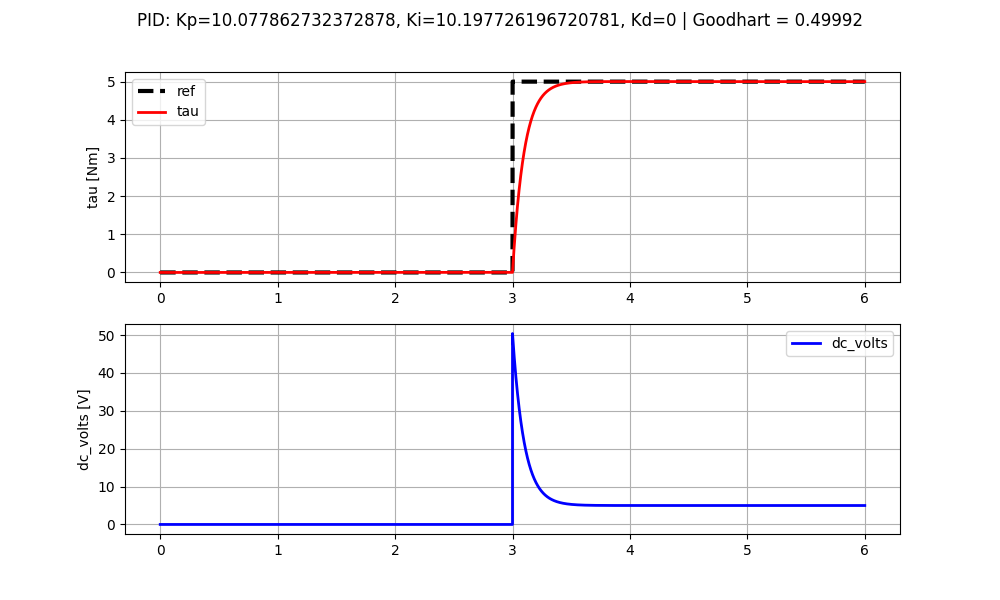
\includegraphics[width=11cm]{pso_degrau_gm.png}
\end{center}

\begin{verbatim}
Tempo total de execução: 1484.252 segundos
Melhor solução encontrada:
Kp = 10.0779
Ki = 10.1977
Kd = 0
Custo = 0.499923
\end{verbatim}

Nesta condição, o PSO também encontra um controlador fortemente proporcional–integral, com desempenho comparável ao do GA e de Nelder--Mead quando se prioriza o termo de erro. O custo é ligeiramente inferior (Goodhart $\approx$ 0.50), ao custo de maior tempo computacional.

\end{document}
